\section{Case Study: Publication Data}
\label{sub:ts-pub}
The previous section demonstrates how TimeSets can support intelligence analysis. This section will discuss an application of TimeSets in a different domain: publication data. A subset containing 200 articles with the most citations from the IEEE InfoVis conference is used~\cite{Stasko2013}. Each publication includes one or many \emph{concepts} such as \emph{network} or \emph{evaluation}, which are used as the \emph{set} attribute for TimeSets to group publications. \autoref{fig:citations} shows the visualization of this dataset. Note that no aggregation is needed when producing the layout; only complete and trimmed labels are used.

\begin{figure}[!htb]
\centering
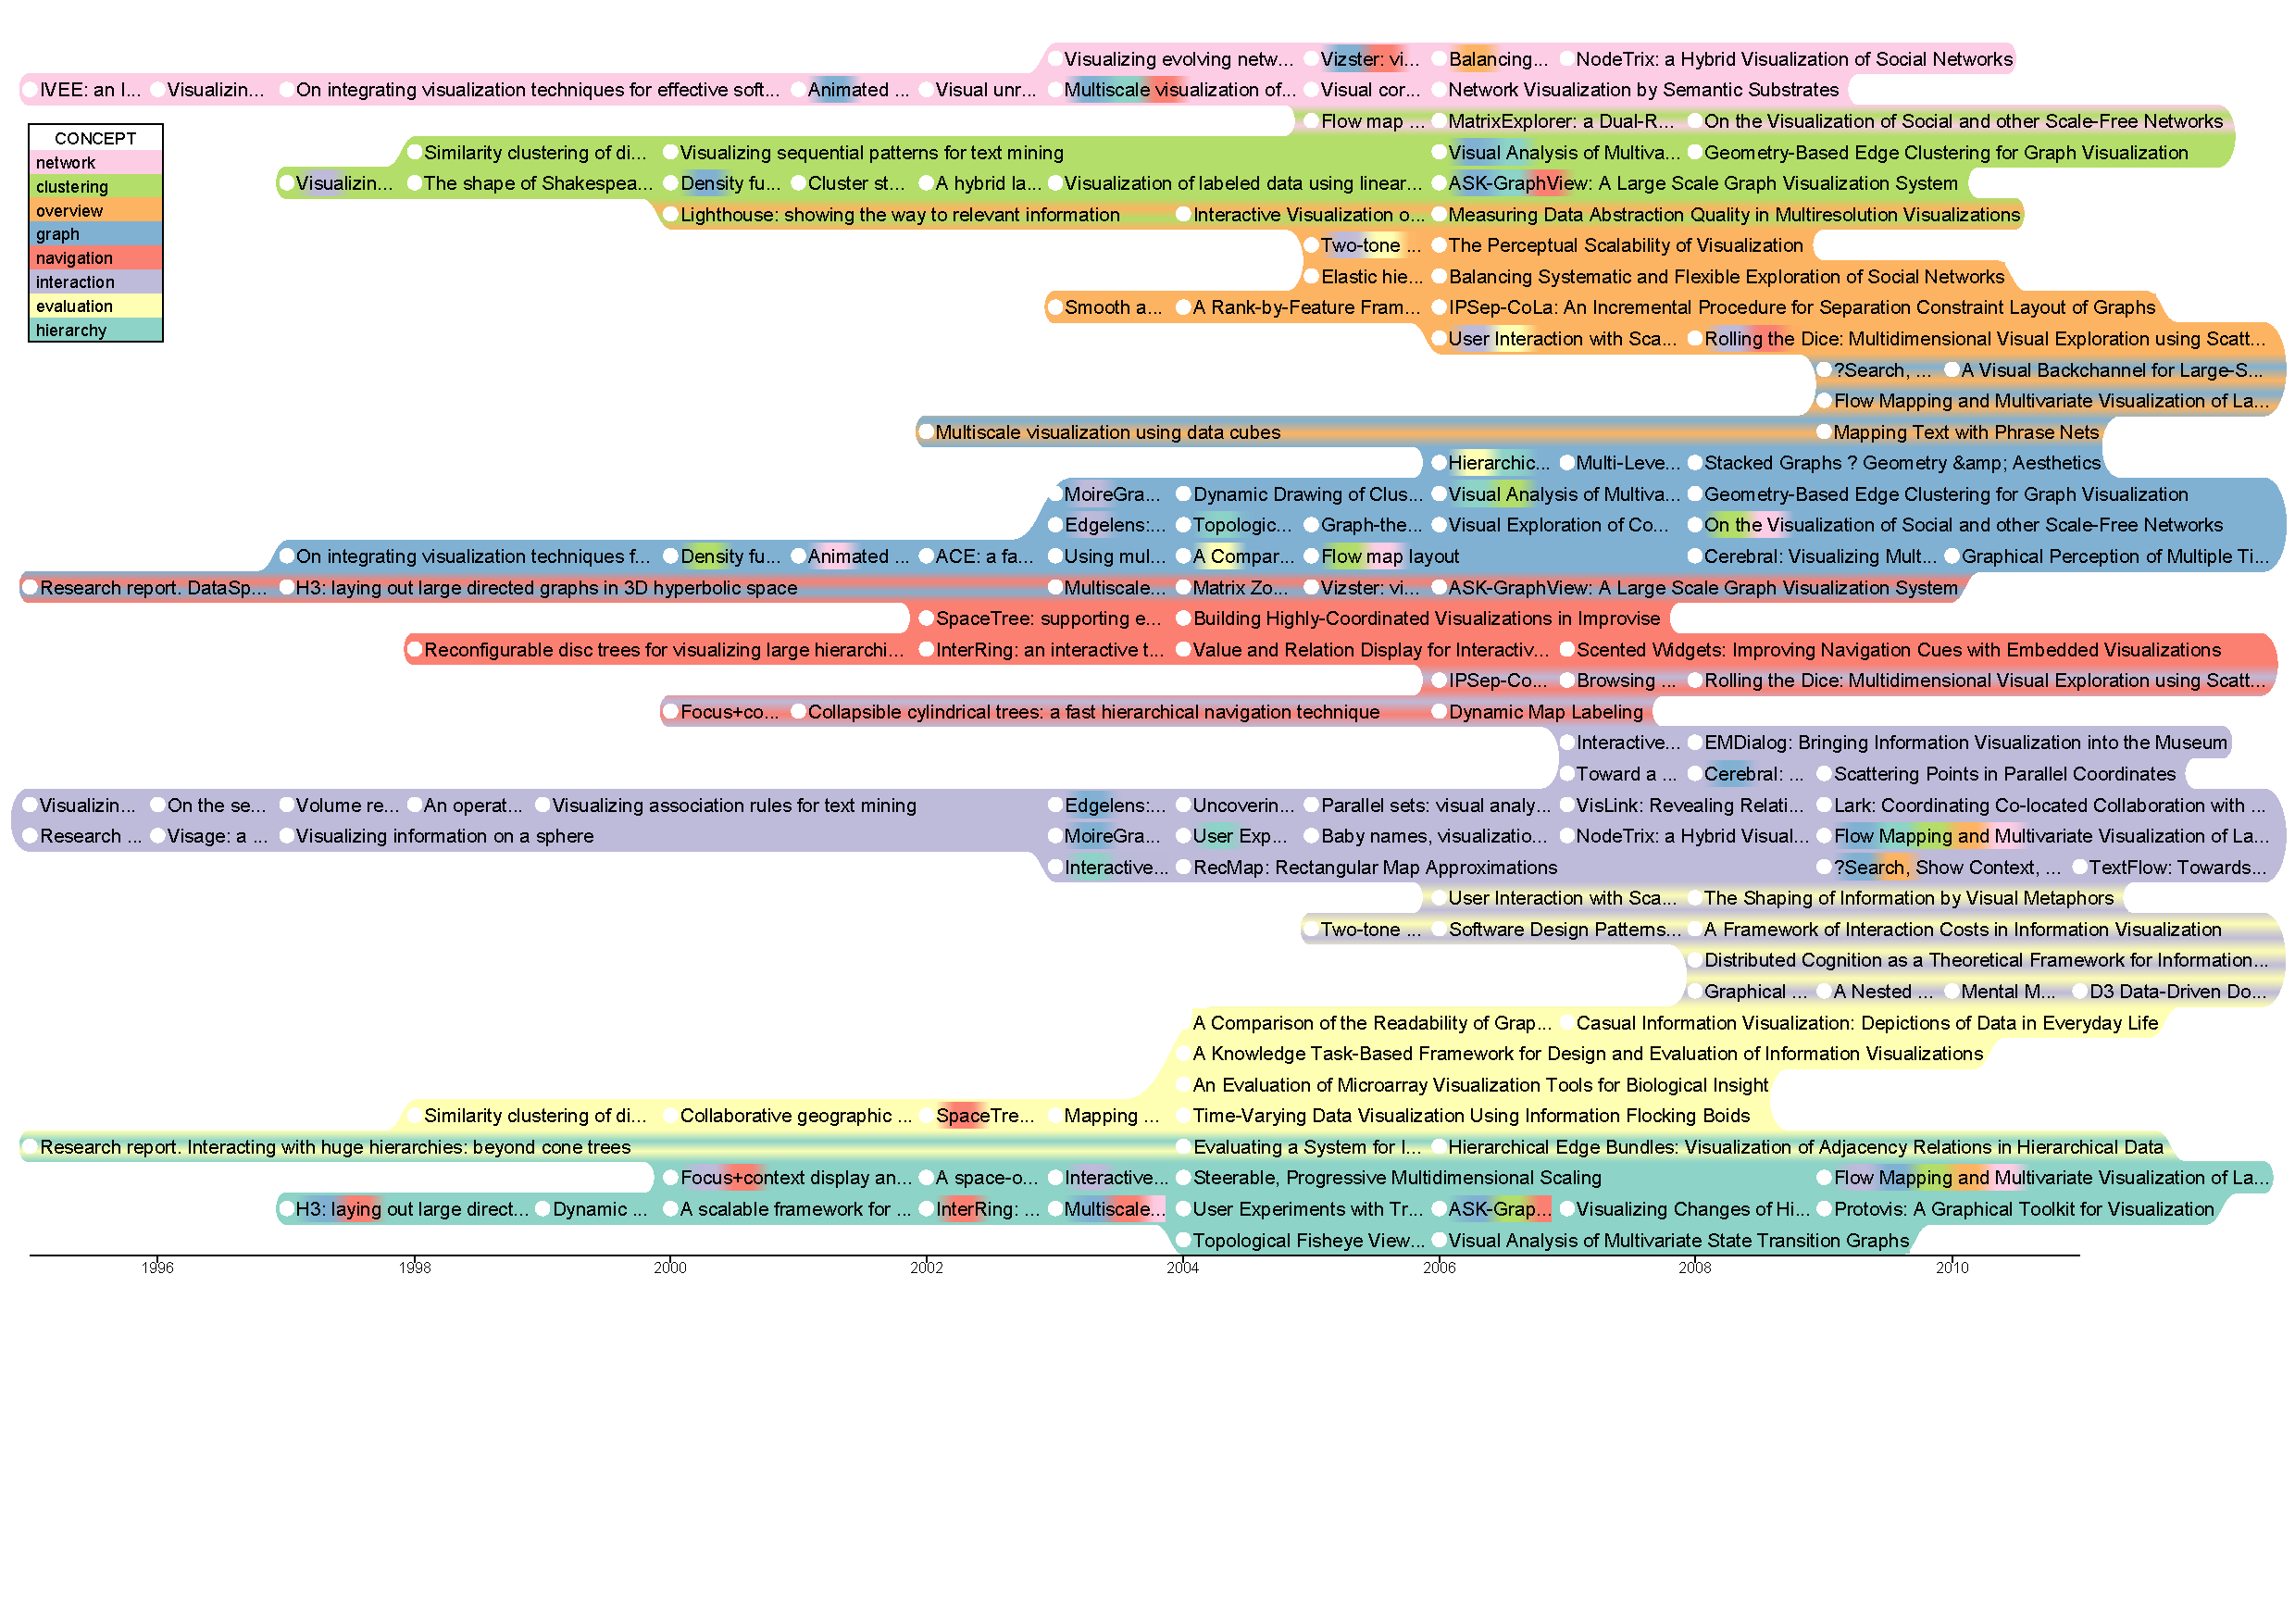
\includegraphics[width=\linewidth]{figure13}
\caption{TimeSets visualization of publication data. It shows 200 articles with the most citations in the IEEE InfoVis conference from 1995 to 2013. These articles are categorized based on their concepts (see the legend in the top left hand corner).}
\label{fig:citations}
\end{figure}

The TimeSets visualization of this publication dataset provides some interesting observations. First, TimeSets can reveal the temporal distribution of a thematic dataset as in ThemeRiver~\cite{Havre2002}. A quick glance at the visualization brings us a surprise. There is much void space on the left as opposed to a very dense area on the right indicating that there are many more highly cited papers published in the last ten years than those in the first ten years. This trend also holds for individual concepts: each colored layer starts with a single row and becomes higher towards the end of the timeline. This observation is in contrast with a common thought: the older the articles are, the more citations they would receive. One possible explanation is that the IEEE InfoVis conference has accepted more papers over time: in the dataset, 18 articles were published 1995, whereas 37 articles were published in 2013. Also, articles in the last ten years are of real high quality.

TimeSets cannot show all intersections among sets; however,  its layout maximizes the number of shared elements between two neighboring sets. Therefore, the visible intersections could include the most elements of all intersections. In \autoref{fig:citations}, the most notable gradient area is the intersection between the yellow set and the purple set indicating that many excellent articles focus on both \tsevaluation{} and \tsinteraction. Also, at the top of the visualization, \tsclustering{} is in between\tsnetwork and \tsoverview{}. This could be because clustering techniques are often used in visualizing large networks and providing an overview of a large dataset.

In \autoref{fig:citations}, TimeSets uses the color gradient method to show full memberships of multi-set elements. An interesting observation is that inside the \tsnetwork{} layer, there are quite a few small blue gradients for \tsgraph. This makes sense because these two concepts may be used interchangeably. We also notice an article including the most concepts at the bottom of the visualization: ``Flow Mapping and Multivariate Visualization...'' (the last article on the third last row) with \tshierarchy, \tsinteraction, \tsgraph, \tsoverview{} and \tsnetwork.

Originally, TimeSets is designed for supporting sensemaking in intelligence analysis. However, this section shows that it can also be used effectively to make sense of data in a different domain -- publication. For an overview, TimeSets helps reveal the evolution of concepts discussed in articles and their relationship over time. For a closer investigation, it helps examine articles chronologically for a particular topic or a group of them.